\section{Database}
Nello sviluppo di un database la prima scelta da compiere è quella relativa al DBMS che si occupa di gestire e garantire l'accesso al database; per questo progetto ho scelto SQLite3 \cite{SQLite3} in quanto in questo caso il DBMS non si basa sull'architettura client-server ma viene direttamente incluso nel programma che s'interfaccia con il database, ciò rende la configurazione quasi automatica. Nel caso specifico di Rius.Co. il database è generato tramite la tecnologia Entity Framework Core sviluppata da Microsoft che pone un ulteriore livello di virtualizzazione tra l'utente e il DBMS che quindi non comunicheranno direttamente tra loro. SQLite3 è conosciuto soprattutto per la sua portabilità in quanto il database è contenuto in un singolo file che risulta molto leggero e compatto, inoltre è anche compatibile con la maggior parte dei sistemi operativi presenti sul mercato. 
\medskip

Per garantire la semplicità di gestione e la velocità di esecuzione delle query nel database sono presenti solo 3 tabelle: Users, Products e Transactions. Queste sono il minimo indispensabile per la creazione di un e-commerce funzionante. Quella riportata nel modello E/R è la prima versione del database che permette di caricare un'unica immagine per prodotto, nelle versioni successive verranno introdotti aggiornamenti graduali paralleli allo sviluppo completo del sito web. Il database è visualizzabile insieme a tutto il progetto scaricando la repository di GitHub \href{https://github.com/MauroPello/elaborato}{disponibile qui} \cite{GitHub}. 
\medskip

La tabella Users contiene le informazioni base necessarie per l'utilizzo della piattaforma: codice identificativo, nome utente, password, email identificativa, città di residenza, immagine di profilo, salt per la generazione dell'hash della password, api key per eseguire richieste tramite l'API e quantità di green coin posseduti. 
\medskip

La tabella Products contiene invece i seguenti campi: codice identificativo, nome, breve descrizione, immagine rappresentativa, disponibilità (per tenere traccia dei prodotti anche dopo la loro vendita o rimozione dal Marketplace), data dell'ultimo aggiornamento apportato e codice identificativo dell'utente proprietario del prodotto. 
\medskip

La tabella Transactions contiene le transazioni effettuate tra gli utenti descritte attraverso i seguenti campi: codice identificativo della transazione, codice identificativo del prodotto scambiato, codice identificativo dell'utente proprietario del prodotto al momento dello scambio (campo necessario per tenere traccia dei cambi di proprietà e delle transazioni anche dopo che queste si sono concluse), codice identificativo dell'utente acquirente, stato della transazione ("In Corso", "Completata Con Successo" o "Completata Senza Successo") e data dell'ultimo aggiornamento relativo alla transazione. 
\subsection{Modello E/R}
\begin{figure} [ht]
    \centering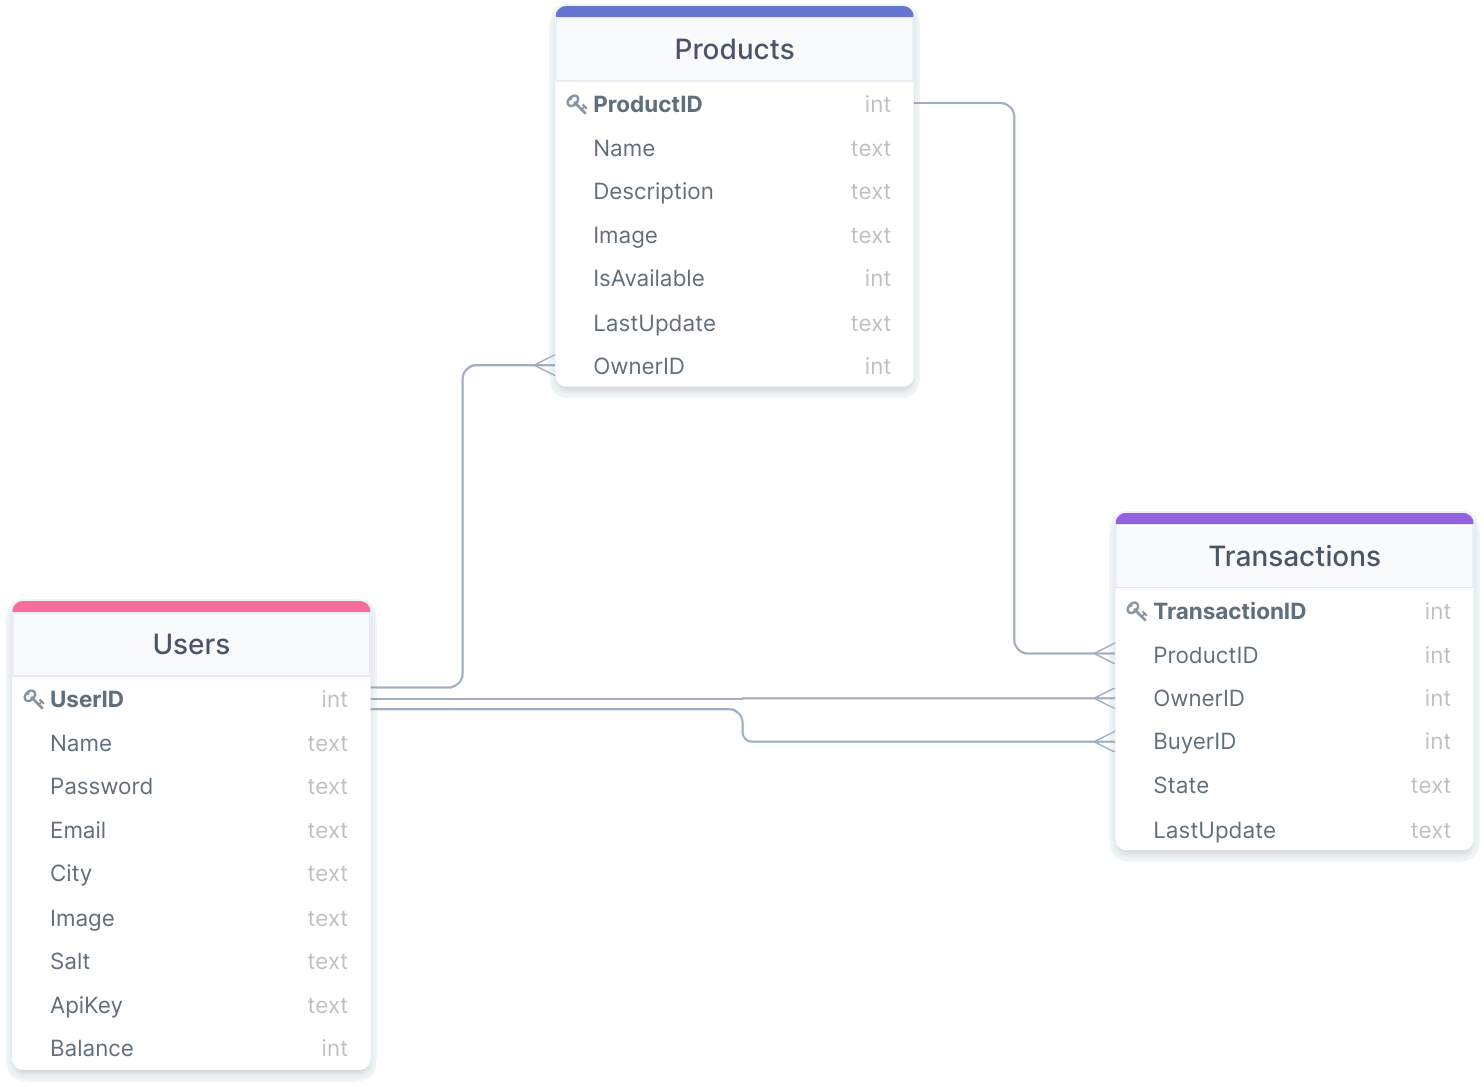
\includegraphics[scale=0.29]{images/modello_e_r.png}
    \caption{Modello E/R sviluppato tramite la web app \href{https://drawsql.app}{disponibile qui} \cite{DrawSQL}.}
\end{figure}
\subsection{Modello logico}
\begin{center}
    \begin{tabular}{ |l|c|l| } 
    \hline
    \multicolumn{3}{|c|}{\large\textbf{Users}} \\
    \hline
    \textbf{Nome Campo} & \textbf{Tipo} & \textbf{Note} \\
    \hline
    UserID & INTEGER & NOT NULL, PK, AUTOINCREMENT \\
    Name & TEXT & NOT NULL \\
    Password & TEXT & NOT NULL \\
    Email & TEXT & NOT NULL \\
    City & TEXT & NOT NULL \\
    Image & TEXT & NOT NULL \\
    Salt & TEXT & NOT NULL \\
    ApiKey & TEXT & NOT NULL \\
    Balance & INTEGER & NOT NULL \\
    \hline
    \end{tabular}
\end{center}
\begin{center}
    \begin{tabular}{ |l|c|l| } 
    \hline
    \multicolumn{3}{|c|}{\large\textbf{Products}} \\
    \hline
    \textbf{Nome Campo} & \textbf{Tipo} & \textbf{Note} \\
    \hline
    ProductID & INTEGER & NOT NULL, PK, AUTOINCREMENT \\
    Name & TEXT & NOT NULL \\
    Description & TEXT & NOT NULL \\
    Image & TEXT & NOT NULL \\
    IsAvailable & INTEGER & NOT NULL \\
    LastUpdate & TEXT & NOT NULL \\
    OwnerID & INTEGER & NOT NULL, FK(Users) \\
    \hline
    \end{tabular}
\end{center}
\begin{center}
    \begin{tabular}{ |l|c|l| } 
    \hline
    \multicolumn{3}{|c|}{\large\textbf{Transactions}} \\
    \hline
    \textbf{Nome Campo} & \textbf{Tipo} & \textbf{Note} \\
    \hline
    TransactionID & INTEGER & NOT NULL, PK, AUTOINCREMENT \\
    ProductID & INTEGER & NOT NULL, FK(Products) \\
    OwnerID & INTEGER & NOT NULL, FK(Users) \\
    BuyerID & INTEGER & NOT NULL, FK(Users) \\
    State & TEXT & NOT NULL \\
    LastUpdate & TEXT & NOT NULL \\
    \hline
    \end{tabular}
\end{center}
\subsection{Entity Framework Core}
Per la creazione del database ho scelto Entity Framework Core, una versione semplice, estendibile, open source e cross-platform della tecnologia di accesso ai dati di grande diffusione chiamata Entity Framework  \cite{EFcore}. Questa tecnologia sviluppata direttamente da Microsoft permette agli sviluppatori di creare e gestire database tramite oggetti scritti in C\# che prendono il nome di modelli, è inoltre compatibile con numerosi DBMS tra cui SQLite3 che è quello adottato in questo progetto. Entity Framework Core supporta anche il versioning del database attraverso l'uso delle migrazioni: gli sviluppatori possono fare modifiche allo schema del database per poi eseguirne successivamente il rollback nel caso non fossero più desiderate. 
\medskip

I database vengono quindi generati automaticamente partendo dai modelli inseriti nel DbContext che descrive il database e le tabelle che lo compongono. Il DbContext da usare viene indicato nel file Startup.cs insieme alla stringa di connessione usata da Entity Framework Core per collegarsi al database. I modelli invece si occupano di descrivere le entità che formano il database, all'interno di questi vengono quindi riportati tutti i campi appartenenti alle tabelle. La nomenclatura dei modelli comprende l'espressione DTO (Data Transfer Object \cite{DTO}) in quanto questi oggetti vengono usati per il trasferimento dei dati dagli utenti al database all'interno del sistema distribuito sul quale è basata la piattaforma. 
\bigskip
\clearpage
\textbf{MainDbContext.cs}
\lstinputlisting[style=csharp]{content/code/MainDbContext.cs}
\bigskip

\textbf{UserDTO.cs}
\lstinputlisting[style=csharp]{content/code/UserDTO.cs}
\bigskip

\textbf{ProductDTO.cs}
\lstinputlisting[style=csharp]{content/code/ProductDTO.cs}
\bigskip

\textbf{TransactionDTO.cs}
\lstinputlisting[style=csharp]{content/code/TransactionDTO.cs}

\subsection{Query}
Usando Entity Framework Core per la creazione e la gestione del database le query possono essere scritte con la sintassi sviluppata da Microsoft chiamata LINQ (Language Integrated Query), questa sintassi ha il vantaggio che è direttamente integrata nel linguaggio C\# \cite{LINQ}. Alternativamente possono essere usati anche i metodi appositi inclusi nella libreria Microsoft.EntityFrameworkCore \cite{Microsoft.EFcore}, questi metodi si occupano di recuperare i dati dal database, modificare quelli già presenti ed eseguire query complesse. Entrambe le modalità per l'esecuzione delle query possono lavorare in modo asincrono, ciò rende Entity Framework Core perfetto per l'ambiente web. Nel progetto ho scelto di usare la libreria Microsoft dedicata in quanto è la più veloce e quella che richiede meno l'intervento del programmatore, evitando quindi errori semplici di distrazione o tempo perso ad ideare query inutilmente complesse. 
\clearpage
\textbf{Query scritta con la sintassi LINQ}
\lstinputlisting[style=csharp]{content/code/linq.cs}
\bigskip
\bigskip

\textbf{Query con i metodi appartenenti alla libreria Microsoft}
\lstinputlisting[style=csharp]{content/code/libreria.cs}